\section*{Aufgabe 5}

Es sei $R$ die folgende Ordnungsrelation auf der Menge $\mathbb{N}^2$:\\
$(x,y) \ R \ (x',y') \Leftrightarrow x \leq x' \text{ und } y \leq y'$\\

a) Man zeige, dass $R$ eine nichtlineare Ordnungsrelation auf $\mathbb{N}^2$ ist.\\

\textit{Linear bedeutet $\forall a,b \in A : aRb \ \lor \ bRa$ somit bedeutet nicht linear $\exists a,b \in A : \lnot aRb \ \land \ \lnot bRa$. Zwei Elemente aus $B$ auf die das zutrifft sind $(1,2)$, $(2,1)$.}\\

b) Für die Menge $B = \{ (1, 3), (1, 2), (2, 1), (2, 2), (2, 3) \}$ bestimme man, falls existent, maximale, minimale Elemente, größtes und kleinstes Element, Supremum und Infimum. Zeichnen Sie das Hasse-Diagramm von $B$ bzgl. der Relation $R$.\\

\textit{Maximales Element:}\\
\textit{$(2,3)$}\\

\textit{Minimales Element:}\\
\textit{$(1,2), (2,1) \rightarrow$ stehen nicht in Relation, können somit nicht verglichen werden}\\

\textit{Größtes Element:}\\
$(2,3)$\\

\textit{Kleinstes Element:}\\
\textit{Existiert nicht, $(1,2)$ und $(2,1)$ stehen nicht in Relation, sind also nicht vergleichbar. Somit kann man nicht alle Element vergleichen um herrauszufinden, welches das kleinste Element ist.}\\

\textit{Infimum:}\\
\textit{$(1,1)$ da wir $(1,2)$ und $(2,1)$ nicht vergleichen können und dies das nächst kleinere untere Grenze ist. Das $(1,1)$ nicht in $B$ ist spielt hierbei keine Rolle.}\\

\textit{Supermum:}\\
$(2,3)$

\begin{figure}[h]
\centering
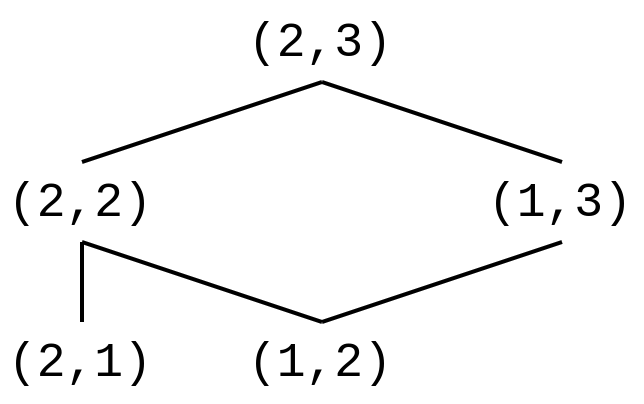
\includegraphics[width=0.3\textwidth]{graphics/hasse.png}
\caption{Hasse-Diagram}
\end{figure}

c) Man gebe eine beschränkte Teilmenge von $\mathbb{N}^2$ an, die kein größtes und kein kleinstes Element besitzt.\\

$\mathbb{N}^2 = \{ (1,2), (2,1), (1,3), (2,2) \}$